%Obviously dates, names, and geography are nowhere near final at this point.

\index{Albion}

	Albion is a nation with territory consisting primarily of the island of Albia, of western Ullr. (fig. \ref{fig:albia})  The island takes its name from the state, rather than vice versa, "Albion" originally being a dynastic name of sorts, describing a kingdom that originated from the mainland.  Although Albion was forced to migrate across the East Sea against its will some thousand years ago, this proved to be fortuitous, as the relative isolation and hospitable terrain preserved the nation.  Many of its contemporaries, lacking the natural defense the sea provided, fell to the sword of invaders.  Albion expanded into the vacuum their demise created, which facilitated the rise of one of the greatest empires of the Middle and Imperial eras.\smallskip \\ 
	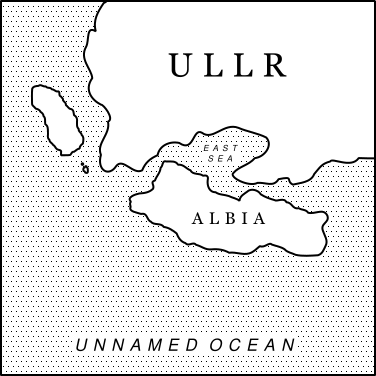
\includegraphics[width=\linewidth]{encyclopedia/images/albia}
	\captionof{figure}{Albia shown in relation to western Ullr.}
	\label{fig:albia}

	\smallskip

	Albion has been best known as one of the two founding members of the East Sea Commonwealth, for its extensive new world colonial empire, and for the invention of the railway.
	
\subsection{History} \index{Albion!History of}
	
	\paragraph{Early History}
	Albion is the sole survivor of four sister kingdoms, the other three being Elbion, Sertion, and Marion.  Evidence for the existence of the other three states is readily available, however the popularly believed story of their origin is unverified and considered legend by most historians.

	\textit{``The king of the realm had four sons.  In order to preserve the peace between his sons upon his death, he ordered that his realm be split in four, with one kingdom given to each son.  The eldest was granted the largest amount of land, named the Kingdom of Marion, and the youngest was granted the smallest kingdom, the Kingdom of Albion.  For a time, there was peace.  However, despite its small size, Albion grew richer and more powerful than the other three brothers.  Eventually the three became tired of being overshadowed by Albion, led by Marion they attempted to destroy Albion out of jealousy.  Albion avoided destruction by crossing the water, and in doing so saved the Albian nation from destruction at the hands the other three did not foresee.''} -Albian Legend

	The final words of the story refer to the invasion of the three remaining kingdoms by numerous groups of Voromen who migrated south.  Their incursions were typically violent and over their course they led to the collapse of Marion, Sertion, and Elbion.  Many refugees escaped to Albion by sea, the Voromen not being mariners, however the majority of the ethnically Albian population remained on the mainland, living under Voromen rule.

	\paragraph{Exile}

	Albion had little difficulty recovering from its setback thanks to the habitability of Albia.  Unlike the Voromen, the Albians were a very maritime culture, and had no trouble adapting to their new life on an island.  Additionally, Albia was already inhabited with small numbers of ethnic Albians, who had moved there over the course of the preceding centuries, and had formed independent villages.  Many of these villages readily became subjects of Albion.  Others banded together to form petty kingdoms in response to the arrival of Albion, and a few small wars were fought on Albia between the 1st and 3rd centuries.  However, none of the petty kingdoms ever approached the strength of Albion, and most were absorbed into Albion, often peacefully, by the 4th century. 

	\paragraph{Reconquest}

	In 201 AC, Wodenburg, a kingdom adjacent to the Voromen territory to the east, launched a westward invasion with the intention of reclaiming territory they had lost a decade before.  Their campaign ended in disaster thanks to a variety of misfortunes, both on the battlefield and at home.  Wodenburg appealed to Albion for assistance, offering both the chance to reclaim territory that had once been Albian, as well as regular tribute.  Albion accepted the proposal and within a few months launched an invasion of the mainland.  

Thanks to the decentralized nature of the Voromen leadership, they were slow to react to the opening of a new theater, and the two-pronged assault on the part of Albion and Wodenburg quickly proved to be successful.  After approximately two years of war, the Wodenburg frontier was pushed a staggering 700 kilometers west, not including Albion's substantial gains.  All parties involved were exhausted by the war by this point, so in 204 AC a peace treaty was signed.

	\paragraph{East Sea Commonwealth} \index{East Sea Commonwealth!Albion}

	\paragraph{Rise of the Empire}

	\paragraph{Fall of the Empire}

	\paragraph{Modern Albion} %reconsider the name of this section, by 'modern' I mean 'between the collapse of the first empire and the millenium war'


\subsection{Government} \index{Albion!Government}
	
	For most of recorded history, Albion has been governed by a monarch.  Succession was initially hereditary, however an elective succession was instituted to solve a succession crisis circa 370 AC.  Although the system was imperfect, it did prove useful for expanding Albion's influence in neighboring Kingdoms, as the succession code permitted the ascension of foreign royalty to the Albian throne.  In this way, personal unions could be formed, with future monarchs continuing to rule both countries.  The most notable instance of this is the union between Albion and Wodenburg, which is commonly cited as the founding of the East Sea Commonwealth.  It is important to note that this is not a retrospective label- the first recorded use of the name is believed to date back to only a few years after the union was first created.
	
	Historically the Albian monarchy was quite strong, however the same was not necessarily true of the nobility.  Until the 7th century Albion was a nominally feudal society, but this system had  coexisted with a limited civil service since the 2nd century, primarily for the collection of taxes as well as a rudimentary secret police force.  One significant and exclusive (At least until the 9th century) power the nobility held was the right to participate in the election of the Albian monarch.  As with any feudal monarchy, the monarch was beholden to the whims of the nobility.  However, thanks to the lessened reliance on the nobility for income, as well as the intelligence gathering and peacekeeping functions of the organized secret police force, more Albian monarchs angered the nobility and lived to tell the tale than in a typical fedual state.

\subsection{Society}  %idk wtf to even do for this, I'll wait and see what other people do

\subsection{Economy}

	The economy of Albion is heavily industrialized, and Albion places among the world's foremost manufacturers.  Other important industries in Albion include agricultiure, fishing, and mining.

%Todo: write a few more lines, once the as-of-printing world is started to get fleshed out